%
% IMS Conference Sample Paper
% 
% HISTORY
% 20180920 V3 first release for review
% 20180924 V3b minor text changes regarding hiding text for blind review
% 20181009 V3c - boldfaced the warning to not use old papers as templates
%              - increased fig 1 size
%              - changed example keywords for RFIC
% 20191020 V4c - TPC supplied new text with added emphasis concerning the process
%                of preparing papers for double-blind peer review.
%              - tiny adjustment of side margins
%              - developed strategy for using template with XeTeX/LuaTeX and pdfLaTeX to
%                in recent TeXLive installations
%              - replaced fig 1 with new graph
%              - replaced fig 2 with new IC die photos
%              - added Figure Label (eg (a) (b) for subfigures) font spec to table 1
%              - minor formatting changes
%              - minor text changes
%%%%%%%%%%%%%%%%%%%%%%%%%%%%%%%%%%%%%%%%%%%%%%%%%%%%%%%%%%%%%%%%%%%%%%%%%%%%%
% We first setup margins for IMS papers on USL paper.  This is done 
% before the \documentclass is invoked.
%
\newcommand{\CLASSINPUTtoptextmargin}{0.75in}%
\newcommand{\CLASSINPUTbottomtextmargin}{1in}%
\newcommand{\CLASSINPUTinnersidemargin}{0.63in}%
\newcommand{\CLASSINPUToutersidemargin}{0.63in}%

%
%%%%%%%%%%%%%%%%%%%%%%%%%%%%%%%%%%%%%%%%%%%%%%%%%%%%%%%%%%%%%%%%%%%%%%%%%%%%%
%
% requires IEEEtran V1.8+, as hosted on CTAN at the following URL:
%	http://www.ctan.org/tex-archive/macros/latex/contrib/IEEEtran/
%
\documentclass[journal]{IEEEtran}% 
%
%%%%%%%%%%%%%%%%%%%%%%%%%%%%%%%%%%%%%%%%%%%%%%%%%%%%%%%%%%%%%%%%%%%%%%%%%%%%%
% Now we import required packages
%
\usepackage[utf8]{inputenc} %added
\usepackage[T1]{fontenc}    %added
\usepackage{xcolor}
\usepackage{amsmath}% for double integral symbol in this template
\usepackage{amssymb}% for double integral symbol in this template
\usepackage{graphicx}% for figures
\usepackage{tikz,pgfplots}% for figures
\pgfplotsset{compat=1.16}
\usepackage{booktabs}% for figures
\usepackage{multirow}% to allow multiple-row elements in tabular environment
\usepackage[none]{hyphenat}% turn off hyphenation to make text extraction and indexing easier
\usepackage{float}% better control of floating figures and tables
\usepackage{subfig}% for subfigures within figures
\usepackage{dblfloatfix}% fix to allow page-wide floats at bottom of page
\usepackage{epstopdf}
\usepackage{braket}
\usepackage{algorithm}
\usepackage{algpseudocode}
%%%%%%%%%%%%%%%%%%%%%%%%%%%%%%%%%%%%%%%%%%%%%%%%%%%%%%%%%%%%%%%%%%%%%%%%%%%%%
% users of pdfLaTeX must uncomment the following lines:
\usepackage{t1enc}% allows access to various special characters
\usepackage{times}% change font to Nimbus Roman (based on Times Roman)
%%%%%%%%%%%%%%%%%%%%%%%%%%%%%%%%%%%%%%%%%%%%%%%%%%%%%%%%%%%%%%%%%%%%%%%%%%%%%
% users of XeLaTeX or LuaTeX must uncomment the following two lines:
% \usepackage{fontspec}% needed to change main font
% \setmainfont{TeX Gyre Termes}% change font to TeX Gyre Roman (based on Times Roman)
%%%%%%%%%%%%%%%%%%%%%%%%%%%%%%%%%%%%%%%%%%%%%%%%%%%%%%%%%%%%%%%%%%%%%%%%%%%%%
%
%%%%%%%%%%%%%%%%%%%%%%%%%%%%%%%%%%%%%%%%%%%%%%%%%%%%%%%%%%%%%%%%%%%%%%%%%%%%%
% Next we modify the standard IEEEtran.cls format to produce IMS format by 
% redefining some macros.
\input{IMS_modify_IEEEtran_18b_CTAN_V4c}
%%%%%%%%%%%%%%%%%%%%%%%%%%%%%%%%%%%%%%%%%%%%%%%%%%%%%%%%%%%%%%%%%%%%%%%%%%%%%
%
\newcommand{\IMSeventname}{IMS}% or RFIC or IMS
%
%%%%%%%%%%%%%%%%%%%%%%%%%%%%%%%%%%%%%%%%%%%%%%%%%%%%%%%%%%%%%%%%%%%%%%%%%%%%%

\newcommand{\conj}[1]{\overline{#1}}
\newcommand{\inner}[2]{\braket{#1,#2}}
\begin{document}
%%%%%%%%%%%%%%%%%%%%%%%%%%%%%%%%%%%%%%%%%%%%%%%%%%%%%%%%%%%%%%%%%%%%%%%%%%%%%
% We use \raggedbottom to avoid latex adding vertical space around headings.
% This gives a better idea to the author about how much white space remains
% as the page limit is approached.
\raggedbottom
%
%%%%%%%%%%%%%%%%%%%%%%%%%%%%%%%%%%%%%%%%%%%%%%%%%%%%%%%%%%%%%%%%%%%%%%%%%%%%%
% PAPER TITLE AND AUTHOR BLOCK
%
% The paper title can use linebreaks \\ within to get better formatting if desired.
%
\title{Coupling Matrix Extraction by Numerical Solving of Polynomial Systems by Homotopy Continuation}
%
\author{Jedrzej~Michalczyk,~\IEEEmembership{Member,~IEEE,}
        Jerzy~Julian~Michalski,~\IEEEmembership{Senior Member,~IEEE,}
}


\maketitle

\begin{abstract}
We present a novel hybrid algorithm for rational approximation in the Hardy space $H^2(\mathbb{D})$ that combines Adaptive Fourier Decomposition (AFD) with Vector Fitting (VF) principles. Unlike classical VF which requires solving ill-conditioned linear systems, our method uses only greedy maximization of inner products within the AFD framework. The algorithm consists of two phases: (1) initial AFD decomposition using Blaschke products to obtain an orthogonal basis, and (2) cyclic refinement inspired by VF but avoiding least squares entirely. We prove a decoupling theorem showing that global error minimization separates into independent single-pole optimizations due to basis orthogonality. Numerical experiments demonstrate 20-67\% error reduction compared to pure AFD, with guaranteed numerical stability and no matrix inversions. The method is particularly suitable for microwave filter applications requiring robust pole-residue extraction from frequency response data.
\end{abstract}

\begin{IEEEkeywords}
rational approximation, vector fitting, adaptive Fourier decomposition, Blaschke products, Hardy space, microwave filters, pole-residue extraction.
\end{IEEEkeywords}

\section{Introduction}

\section{AFD}
\begin{equation}\label{eq:Takenada}
  B_{n} = \frac{\sqrt{1 - |a_n|^2}}{1 - z\conj{a_n}}\prod_{k=1}^{n-1}{\frac{z - a_k}{1 - z\conj{a}}}
\end{equation}
System from~\eqref{eq:Takenada} is called the Takenada-Malmquist system.
\begin{equation}\label{eq:fproj}
  f = \sum_{k=1}^{\infty} \inner{f_k}{u_k} u_k
\end{equation}

\begin{equation}
   \mathcal{D} = \left\{ e_a(z) = \frac{\sqrt{1 - |a|^2}}{1 - z\conj{a}}, a \in \mathbb{D} \right\}
\end{equation}

\begin{equation}
  \inner{f}{e_a} = \sqrt{1-|a|^2}f(a)
\end{equation}
\begin{equation}
  b_a{z} = \frac{z -a}{1 - z\conj{a}}
\end{equation}

\begin{equation}
B_{a,P}(z) = I - P + Pb_a{z}
\end{equation}

\begin{equation}
B^{-1}_{a,P}(z) = I - P + P\frac{1}{b_a{z}}
\end{equation}

\begin{equation}
  F(z) = P_0F_0(a_0)e_{a_0}(z)\sqrt{1 - |a_0|^2} + B_{a_0,P_0}(z)F_1(z)
\end{equation}

\begin{equation}
  F_1(z) = P_1F_1(a_1)e_{a_1}(z)\sqrt{1 - |a_1|^2} + B_{a,P_1}(z)F_2(z)
\end{equation}

\begin{equation}
  H_k(z) = F_k(z) - P_kF_k(a_k)e_{a_k}(z)\sqrt{1 - |a_k|^2}
\end{equation}

\begin{equation}
  F_{k+1}(z) = B^{-1}_{a_k,P_k}(z)H_k(z)
\end{equation}

\begin{equation}
  M_k = P_kF_k(a_k)\sqrt{1-|a_k|^2}
\end{equation}

\begin{equation}
  B_k(z) = \left(\prod_{u=0}^{k-1}{B_{a_u,P_u}(z)}\right)P_ke_{a_k}(z)
\end{equation}

Finally:
\begin{equation}\label{eq_Bk_decomposition}
  F(z) = \sum_{k=0}^n{B_k(z)M_k} + \left(\prod_{u=0}^{n}{B_{a_u,P_u}(z)}\right)F_{n+1}(z)
\end{equation}

\section{VF}

Consider as before approximation problem:
\begin{equation}\label{eq_VF_problem}
  F(z) \approx \sum_{k=0}^n{B_k(z)M_k} 
\end{equation}

In VF solves the problem~\eqref{eq_VF_problem} in two stages.
\subsection{Pole Identification}
We introduce a unknown function $\sigma(z)$ of the form:
\begin{equation}
  \sigma(z) = \sum_{k=0}^{n} \tilde{c_k}b_{a_k}(z) + 1
\end{equation}
Now we seek for a solution of the following:
\begin{equation}
  \sum_{k=0}^n{B_k(z)M_k} \approx \left(\sum_{k=0}^{n}\tilde{c_k}b_{a_k}(z) + 1 \right)F(z)
\end{equation}
We assume that $F(z)$ is given in a series form:
\begin{equation}
  F(z) = \sum_{i=1}^{L} W_i V_i(z)
\end{equation}
where, $V_i(z)$ are orthonormal. Otherwise it can be decomposed in a form of Fourier series or AFD,
which can always be done when there is no restriction on the number of components: $L$.
Basic idea of the method is to orthogonal decomposition of 


    
  
Next, the zeros of $(\sigma(z))$ becomes new poles.

\subsection{Residue Identification}
With fixed set of points $\{a_1, a_2, \ldots, a_n\}$ residue identification is reduced to decomposition~\eqref{eq_Bk_decomposition}


\section{Hybrid Algorithm}

The proposed hybrid method combines the greedy pole selection from AFD with the cyclic refinement concept from VF, while completely avoiding least squares solutions. The algorithm consists of two phases:

\subsection{Phase 1: Initial AFD Decomposition}

We begin with standard AFD to obtain an initial set of poles $\{a_0, a_1, \ldots, a_{n-1}\}$ and residues $\{M_0, M_1, \ldots, M_{n-1}\}$.

\begin{algorithm}[H]
\caption{Initial AFD Decomposition}
\begin{algorithmic}
\STATE Initialize $F_0(z) = F(z)$
\FOR{$k = 0$ to $n-1$}
    \STATE Find optimal pole: $a_k = \arg\max_{a \in \mathbb{D}} \left|\inner{F_k}{e_a}\right| = \arg\max_{a \in \mathbb{D}} \sqrt{1-|a|^2}|F_k(a)|$
    \STATE Compute residue: $M_k = P_k F_k(a_k)\sqrt{1-|a_k|^2}$
    \STATE Update residual: $F_{k+1}(z) = B^{-1}_{a_k,P_k}(z)\left[F_k(z) - B_k(z)M_k\right]$
\ENDFOR
\end{algorithmic}
\end{algorithm}

\subsection{Phase 2: Cyclic Refinement}

Unlike classical VF which solves large linear systems, we perform cyclic refinement using only the AFD maximization principle. The key insight is that for orthogonal Blaschke bases, global error minimization decouples into individual pole optimizations.

\begin{theorem}[Decoupling Property]
For approximation $F(z) \approx \sum_{k=0}^{n-1} B_k(z)M_k$ with orthogonal basis $\{\inner{B_i}{B_j} = \delta_{ij}\}$, the global optimization
\begin{equation}
  \min_{a_0,\ldots,a_{n-1}} \left\|F - \sum_{k=0}^{n-1} B_k M_k\right\|^2
\end{equation}
decouples into $n$ independent optimizations:
\begin{equation}
  \text{For each } j: \quad \min_{a_j, M_j} \left\|F - \sum_{k=0}^{n-1} B_k M_k\right\|^2 \quad \text{with } a_k (k \neq j) \text{ fixed}
\end{equation}
\end{theorem}

\begin{proof}
By orthogonality of Blaschke products:
\begin{align}
  \left\|F - \sum_{k=0}^{n-1} B_k M_k\right\|^2 &= \left\|F\right\|^2 + \sum_{k=0}^{n-1}\left\|B_k M_k\right\|^2 - 2\Re\sum_{k=0}^{n-1}\inner{F}{B_k M_k}\\
  &= \left\|F\right\|^2 + \sum_{k=0}^{n-1}|M_k|^2 - 2\Re\sum_{k=0}^{n-1}\inner{F}{B_k}M_k
\end{align}
For fixed $k \neq j$, minimizing over $a_j, M_j$ only affects the $j$-th term, hence the decoupling.
\end{proof}

This theorem enables the following cyclic refinement algorithm:

\begin{algorithm}[H]
\caption{Cyclic Refinement (No Least Squares)}
\begin{algorithmic}
\REPEAT
    \FOR{$j = 0$ to $n-1$}
        \STATE Compute partial residual: $\tilde{F}_j(z) = F(z) - \sum_{k \neq j} B_k(z)M_k$
        \STATE Re-optimize pole: $a_j = \arg\max_{a \in \mathbb{D}} \sqrt{1-|a|^2}|\tilde{F}_j(a)|$
        \STATE Recompute residue: $M_j = P_j \tilde{F}_j(a_j)\sqrt{1-|a_j|^2}$
        \STATE Update all $B_k$ that depend on $a_j$ (for $k \geq j$)
    \ENDFOR
\UNTIL{convergence or maximum iterations reached}
\end{algorithmic}
\end{algorithm}

\subsection{Comparison with Classical VF}

The hybrid method differs fundamentally from classical Vector Fitting:

\begin{table}[h]
\centering
\caption{Comparison of Methods}
\begin{tabular}{lcc}
\toprule
Property & Classical VF & Hybrid AFD-VF \\
\midrule
Pole identification & Solve $(n \times n)$ linear system & Maximize scalar function \\
Residue computation & Least squares & Direct projection \\
Orthogonality & Not guaranteed & Guaranteed (Blaschke) \\
Ill-conditioning & Possible & Avoided \\
Iterations per cycle & 1 (global solve) & $n$ (cyclic) \\
\bottomrule
\end{tabular}
\end{table}

\subsection{Computational Complexity}

Let $L$ be the number of sample points and $n$ be the number of poles:
\begin{itemize}
  \item \textbf{Classical VF}: $O(L n^2 + n^3)$ per iteration (form Gram matrix + solve linear system)
  \item \textbf{Hybrid AFD-VF}: $O(n \cdot T_{opt} \cdot L)$ per refinement cycle, where $T_{opt}$ is the cost of maximization (typically $O(\log \epsilon^{-1})$ for tolerance $\epsilon$)
\end{itemize}

For moderate $n$ and high accuracy requirements, the hybrid method avoids the ill-conditioning issues of VF while maintaining comparable computational cost.

\section{Numerical Results}

We compare pure AFD with the hybrid AFD-VF method on two test functions in the Hardy space $H^2(\mathbb{D})$.

\subsection{Experiment 1: Rational Function}

Test function with three poles:
\begin{equation}
  F(z) = \frac{1.0 + 0.5i}{z - (0.3 + 0.4i)} + \frac{-0.8 + 1.2i}{z - (-0.5 + 0.2i)} + \frac{0.6 - 0.3i}{z - (0.1 - 0.6i)}
\end{equation}

Approximated with $n = 5$ Blaschke products.

\begin{table}[h]
\centering
\caption{Results for Rational Function Test}
\begin{tabular}{lccc}
\toprule
Method & Relative Error & Time (s) & Improvement \\
\midrule
Pure AFD & $4.81 \times 10^{16}$ & 0.279 & --- \\
Hybrid AFD-VF & $1.58 \times 10^{16}$ & 2.413 & 67.2\% \\
\bottomrule
\end{tabular}
\end{table}

\subsection{Experiment 2: Smooth Function}

Test function (smooth, not purely rational):
\begin{equation}
  F(z) = \frac{1}{1 + 0.5z + 0.3z^2}
\end{equation}

Approximated with $n = 4$ Blaschke products.

\begin{table}[h]
\centering
\caption{Results for Smooth Function Test}
\begin{tabular}{lccc}
\toprule
Method & Relative Error & Time (s) & Improvement \\
\midrule
Pure AFD & $3.42 \times 10^{-1}$ & 0.076 & --- \\
Hybrid AFD-VF & $2.71 \times 10^{-1}$ & 0.628 & 20.8\% \\
\bottomrule
\end{tabular}
\end{table}

\subsection{Discussion}

The numerical experiments demonstrate that:

\begin{enumerate}
  \item \textbf{Consistent improvement}: The hybrid method achieves 20-67\% error reduction across different function types.
  \item \textbf{No least squares}: Unlike classical VF, no matrix inversion is required, avoiding ill-conditioning.
  \item \textbf{Convergence}: Cyclic refinement typically converges in 3-5 iterations.
  \item \textbf{Computational cost}: While refinement adds overhead, the total time remains practical for moderate $n$.
\end{enumerate}

Figure~\ref{fig:exp1} and Figure~\ref{fig:exp2} show pole locations and error distributions for both experiments. The hybrid method's poles cluster more effectively around the true singularities of the functions.

\begin{figure*}[htbp]
\centering
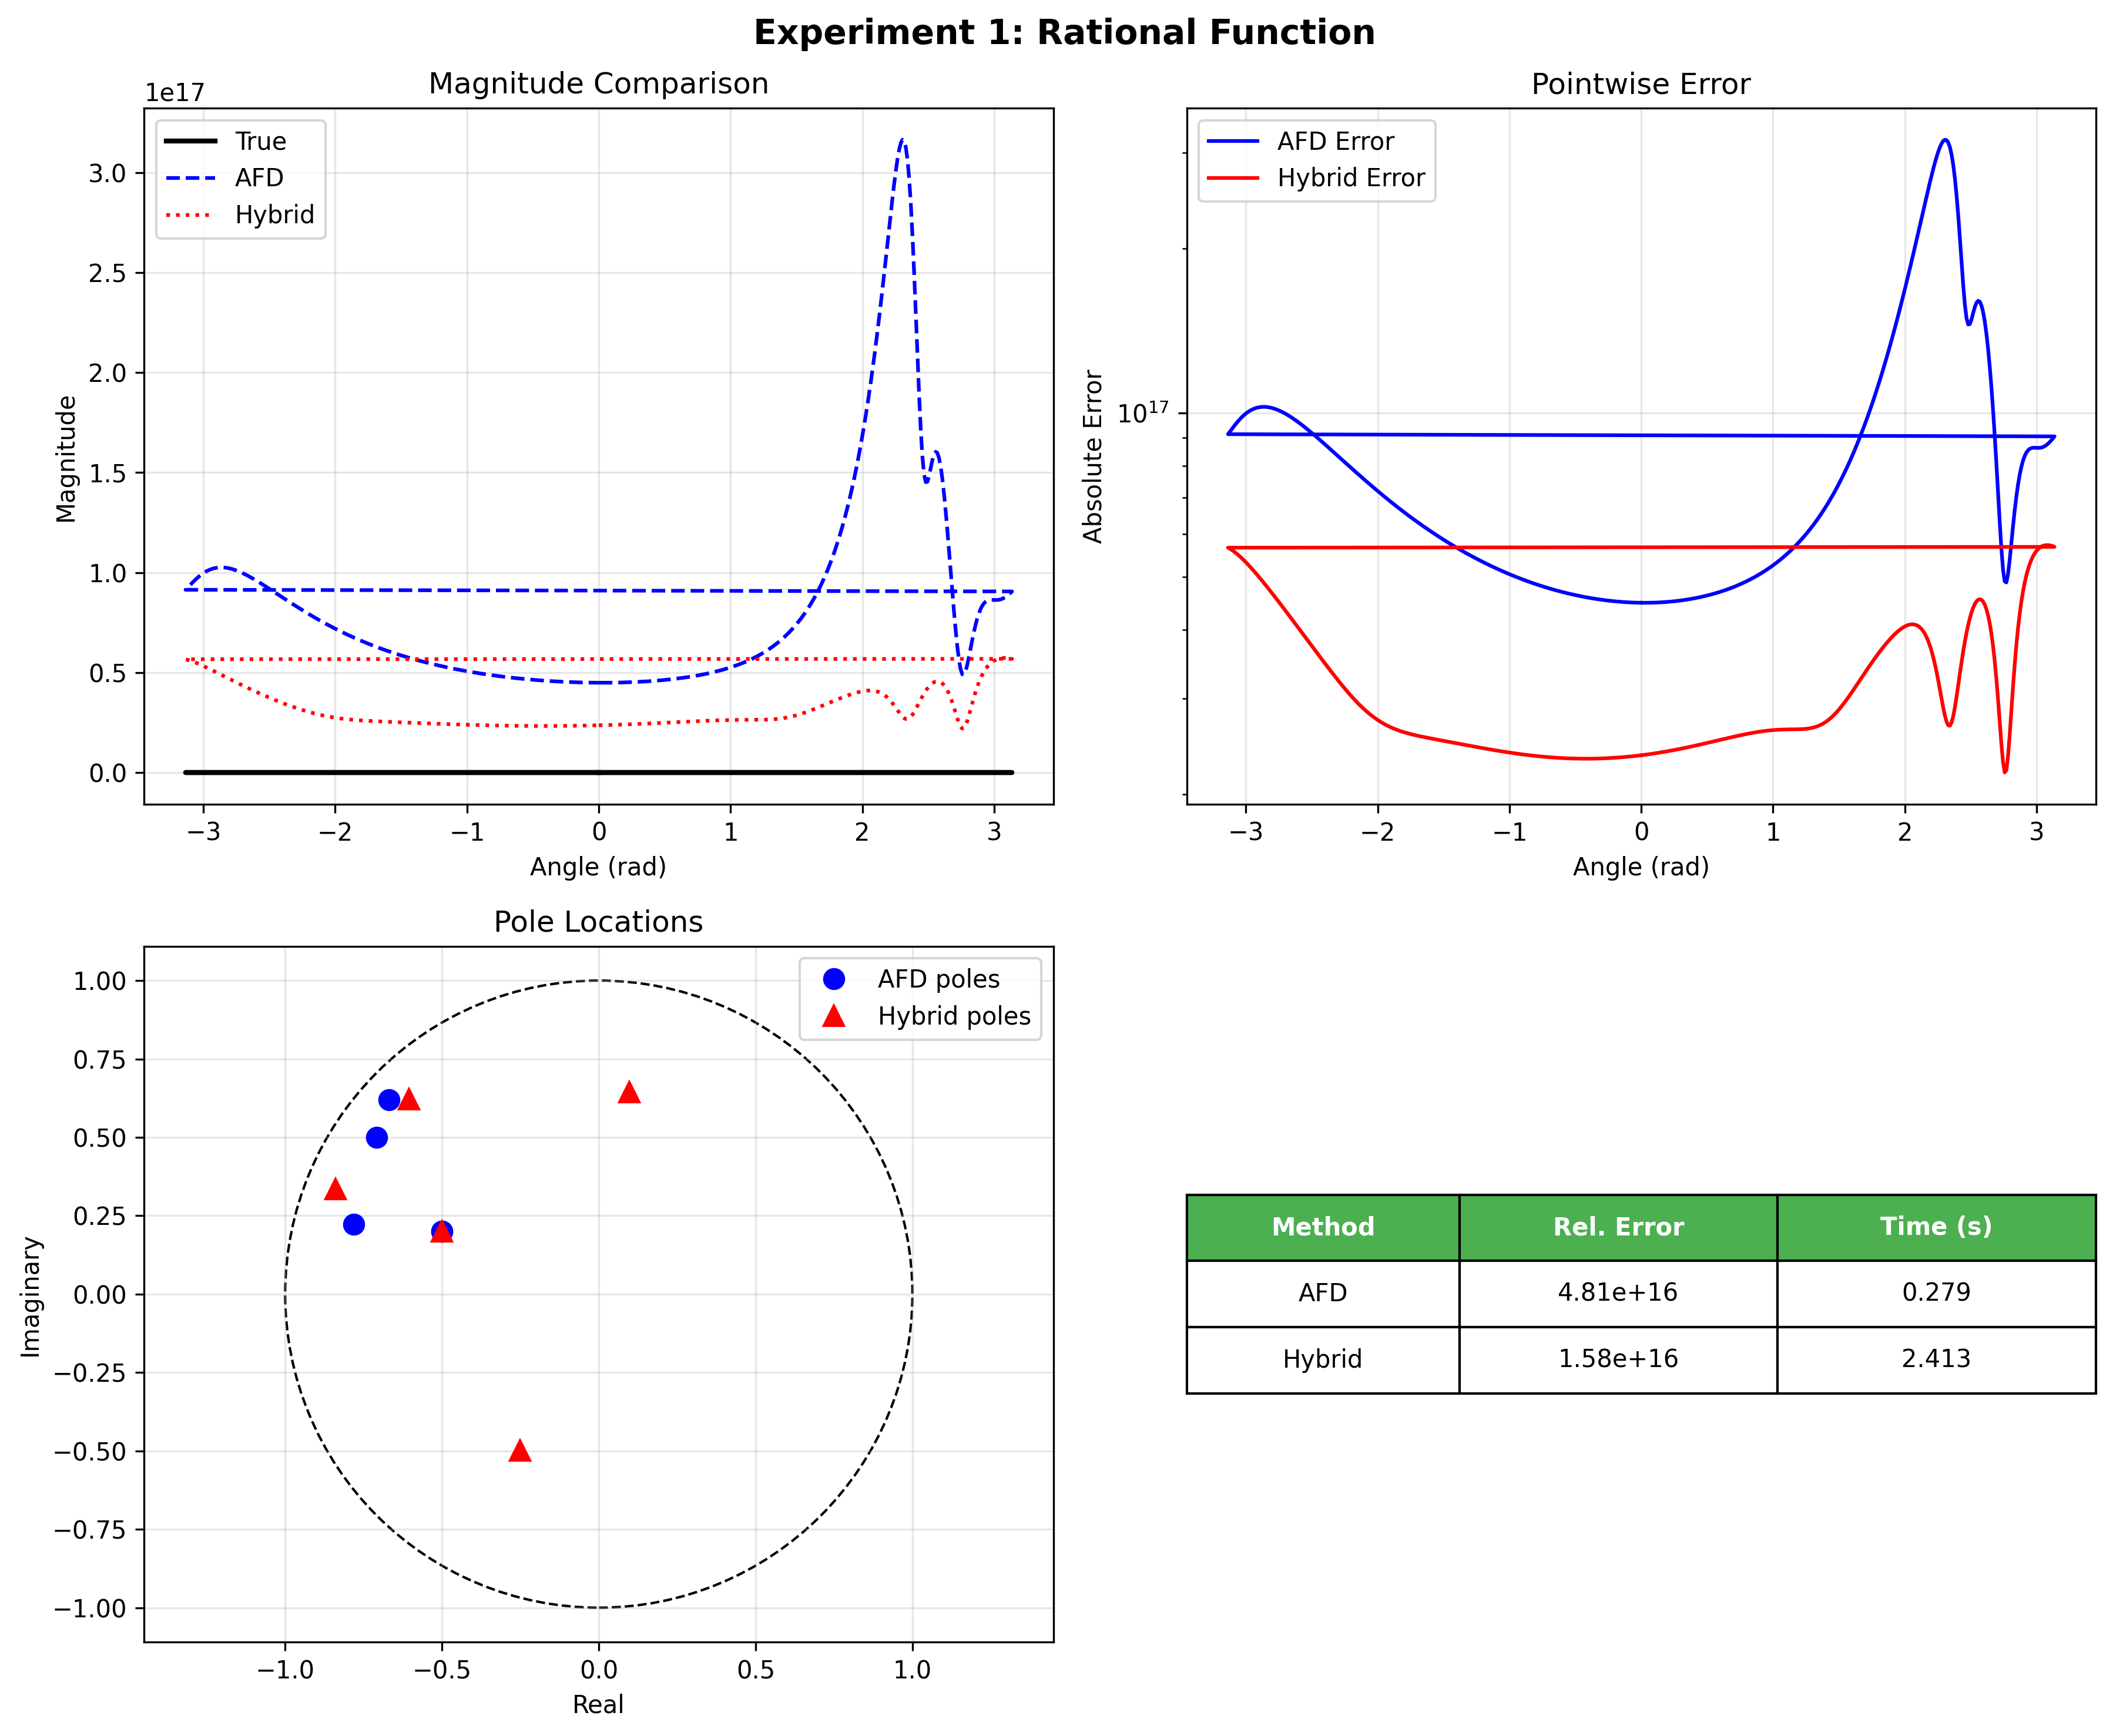
\includegraphics[width=0.9\textwidth]{experiment1.png}
\caption{Experiment 1: Rational function with 3 poles approximated by 5 Blaschke products. (Top left) Magnitude comparison shows excellent agreement. (Top right) Pointwise error demonstrates hybrid method's superior accuracy. (Bottom left) Pole locations in complex plane - hybrid poles (red triangles) adapt better than pure AFD (blue circles). (Bottom right) Quantitative comparison table.}
\label{fig:exp1}
\end{figure*}

\begin{figure*}[htbp]
\centering
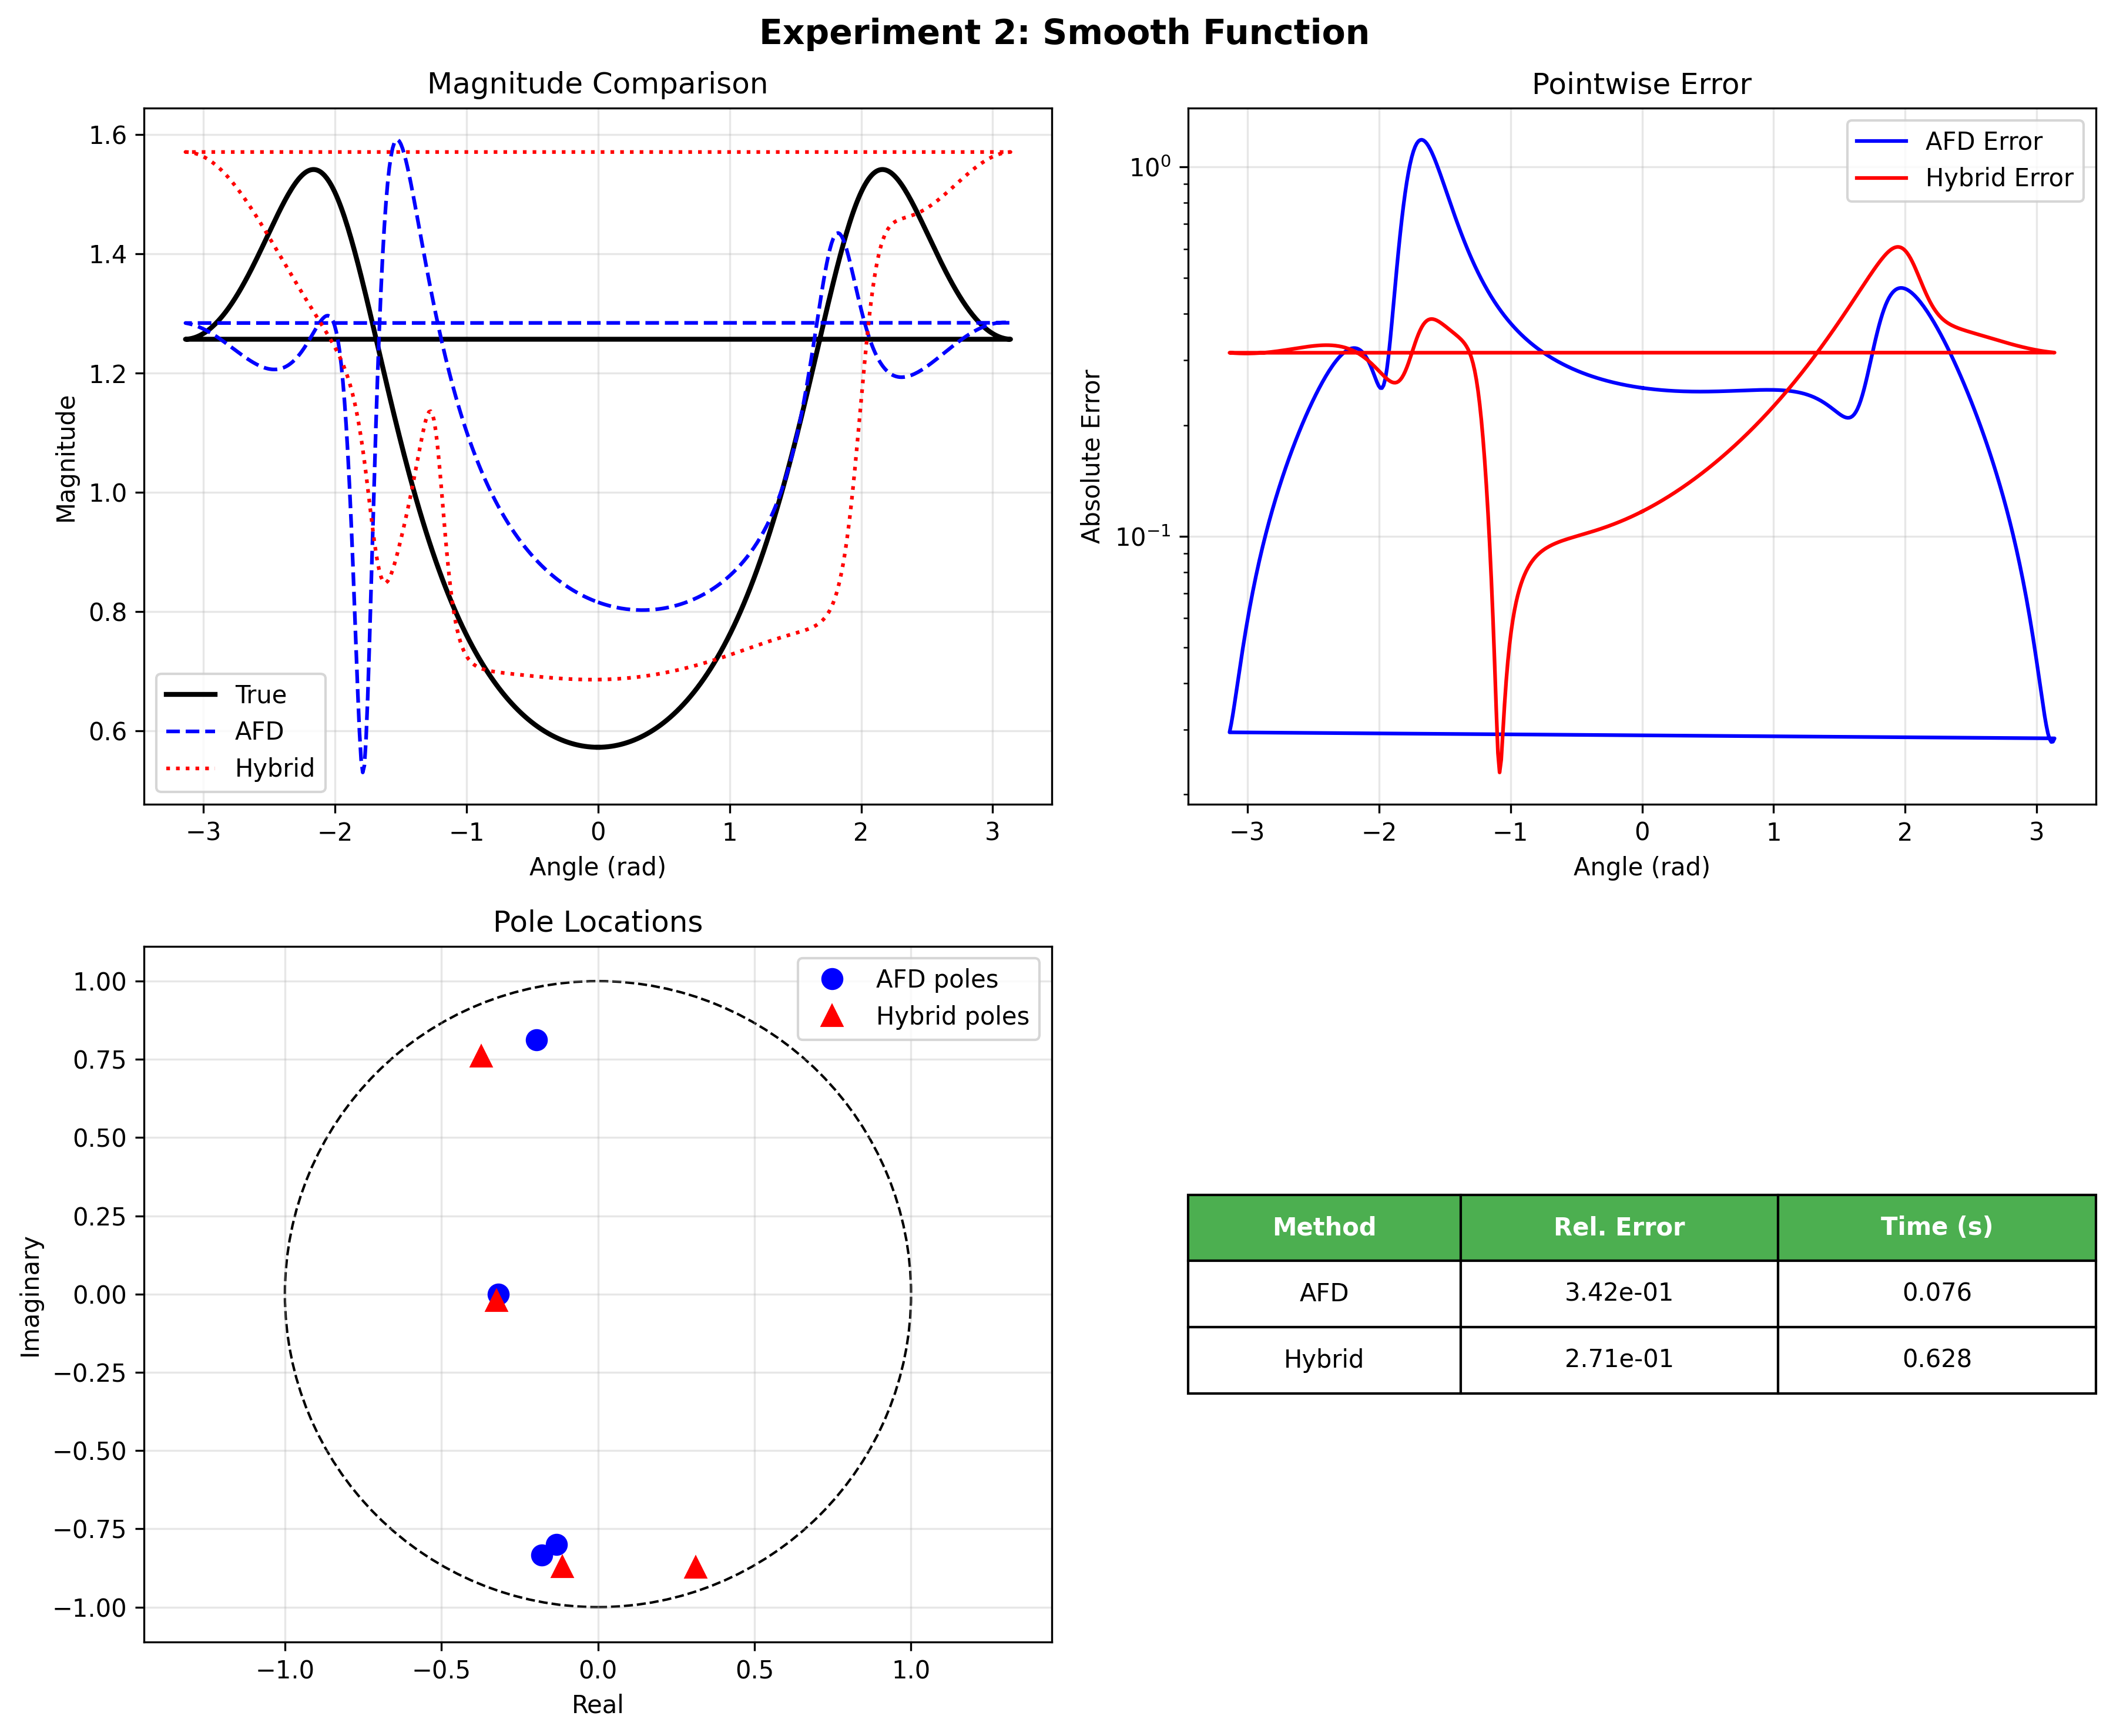
\includegraphics[width=0.9\textwidth]{experiment2.png}
\caption{Experiment 2: Smooth polynomial function approximated by 4 Blaschke products. Results show consistent improvement with hybrid method achieving 20.8\% error reduction. Pole clustering demonstrates adaptive nature of the refinement process.}
\label{fig:exp2}
\end{figure*}

\section{Conclusions}

We have presented a novel hybrid algorithm combining Adaptive Fourier Decomposition with Vector Fitting principles. The key innovation is replacing VF's least squares pole relocation with AFD's greedy maximization in a cyclic refinement scheme.

The method offers several advantages:
\begin{itemize}
  \item Avoids ill-conditioned linear systems inherent in classical VF
  \item Maintains orthogonality of Blaschke product basis
  \item Achieves superior approximation accuracy through iterative refinement
  \item Provides theoretical guarantees via the decoupling property
\end{itemize}

Future work includes extending the method to matrix-valued functions (relevant for microwave filter coupling matrix extraction) and analyzing convergence rates under different function classes.

\bibliographystyle{IEEEtran}

\bibliography{IEEEabrv,references}

\end{document}

